\makeatletter
\makeatother
\documentclass[../main.tex]{subfiles}

\graphicspath{
    {img}
	{../img/}
}

\begin{document}
\section{Метод Римана}

Мы праябаліся і прапусцілі яго :( Таму замест тэха Рымана тут скрыншоты канспекту Лізы

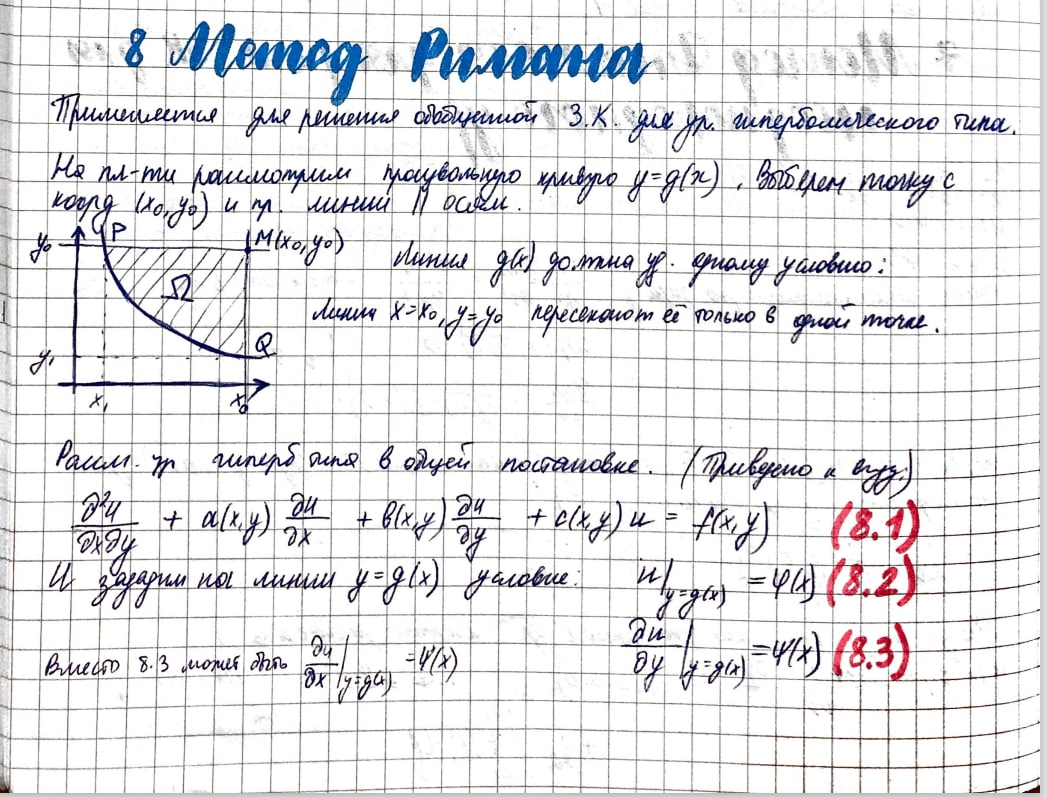
\includegraphics[scale=0.7]{Liza_2.7.1.jpg}
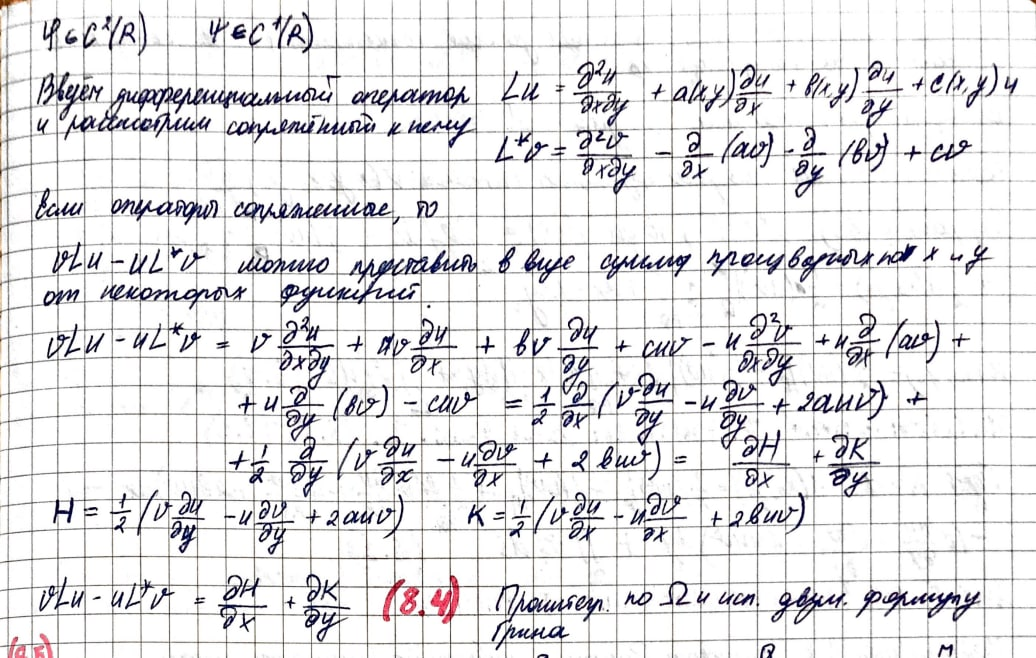
\includegraphics[scale=0.7]{Liza_2.7.2.jpg}
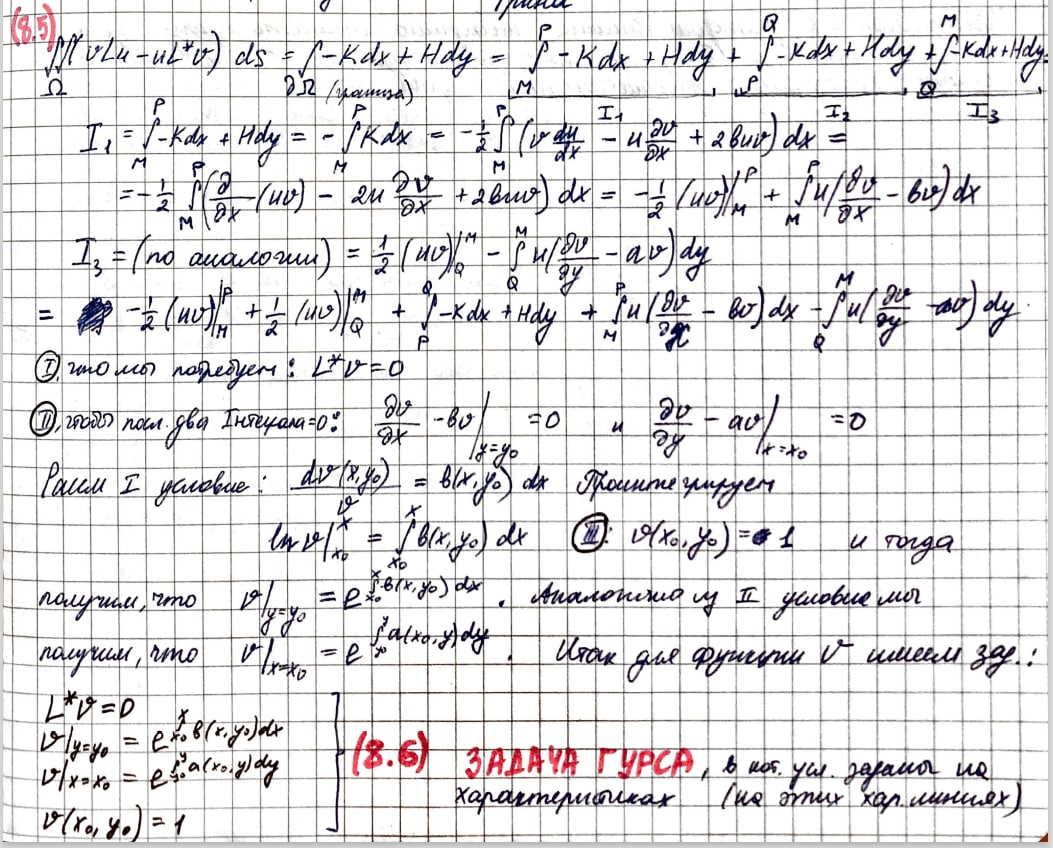
\includegraphics[scale=0.7]{Liza_2.7.3.jpg}
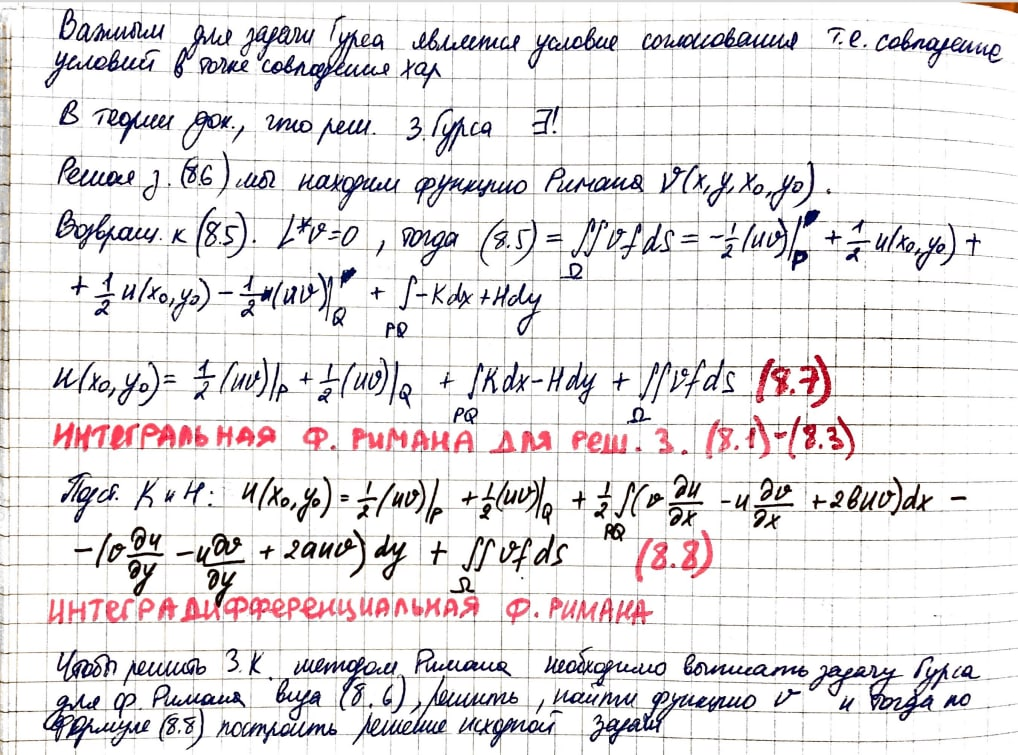
\includegraphics[scale=0.7]{Liza_2.7.4.jpg}
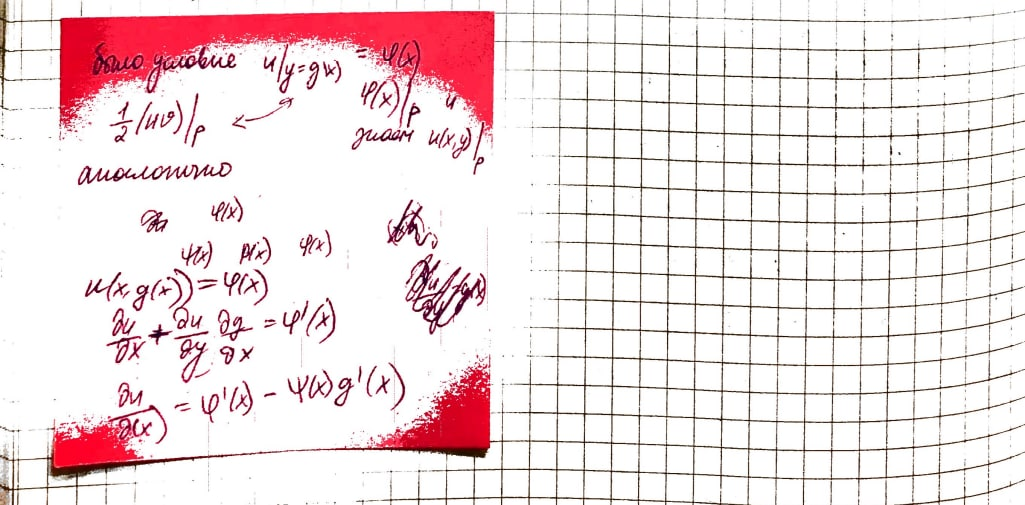
\includegraphics[scale=0.7]{Liza_2.7.5.jpg}

WIP

\end{document}